\documentclass[10pt]{article}
\usepackage{../../local}
\urlstyle{same}

\newcommand{\classcode}{EE 120}
\newcommand{\classname}{Signals and Systems}
\renewcommand{\maketitle}{%
\hrule height4pt
\large{Eric Du \hfill \classcode}
\newline
\large{HW 11} \Large{\hfill \classname \hfill} \large{\today}
\hrule height4pt \vskip .7em
\small{Header styling inspired by CS 70: \url{https://www.eecs70.org/}}
\normalsize
}
\linespread{1.1}
\begin{document}
	\maketitle
	\section*{Collaborators}	
	I worked with the following people on this assignment:
	\begin{itemize}
		\item Teja Nivarthi: 3036508567
		\item Nikhil Maserang: 3036978230
	\end{itemize}
	\pagebreak
	\section*{Problem 1}
	Find the right-sided sequence whose \( z \)-transform is
	\[
	Z(z) = \frac{1 - 2z^{-1}}{1 + \frac{5}{2}z^{-1} + z^{-2}}
	\] 

	\begin{solution}
		Here we use partial fraction decomposition. We can see that here, \( M = 1 \) and \( N = 2 \), 
		so this implies that \( Z(z) \) is of the form:
		\[
		Z(z) = \sum_{k=1}^{N} \frac{A_k}{1 - d_k z^{-1}}
		\] 
		where \( d_k \) are the poles. Here, the roots are \( z = -2, -\frac{1}{2} \), so this means that:
		\[
		Z(z) = \frac{A_1}{1 + 2z^{-1}} + \frac{A_2}{1 + \frac{1}{2}z^{-1}}
		\] 
		Matching the coefficients (multiplying out, solving for \( A_1, A_2 \)), we get \( A_1 = -\frac{5}{3} \), 
		\( A_2 = \frac{8}{3} \). So, now we know the full form of \( Z(z) \). Further, since we want to find 
		the right-sied sequence, this implies that the ROC of this includes infinity, meaning that the 
		sequence \( x[n] \) is given by:
		\[
			x[n] = -\frac{5}{3}(-2)^{n}u[n] + \frac{8}{3}\left( -\frac{1}{2} \right)^{n}u[n]
		\] 
		We know that they must be step functions \( u[n] \) since we're given from the problem statement that the 
		sequence we want to find is right-sided. 
	\end{solution}
	\pagebreak
	\section*{Problem 2}
	In this problem, we examine the locations of the poles and zeroes of prototypical finite-length DT signals. 
	A signal \( x \) is \textit{finite-length} if \( x[n] = 0 \) outside a finite set of samples \( n \). 

	For each of the following real-valued, finite-length discrete-time signals \( r, v \), and \( w \), determine a 
	reasonably simple expression for the corresponding \( z \)-transforms \( \hat{R}(s), \hat{V}(z) \) and 
	\( \hat{W}(z) \), and determine all the pole ocations (ignoring infinite poles). You may treat 
	\( \alpha, \beta \) and \( \gamma \) as constants. 

	\begin{enumerate}[label=\alph*)]
		\item \( r[n] = \alpha \delta[n] + \beta \delta[n - 1] + \gamma \delta[n - 2] \) 

			\begin{solution}
				In all these problems, we use linearity to simplify along with the given \( z \)-transform 
				pairs. Here, this transforms as:
				\[
				\hat{R}(z) = \alpha + \beta z^{-1} + \gamma z^{-2}
				\] 
				The ROC of this is all \( z \) except at \( z = \infty \), but we are asked to ignore that. 
			\end{solution}
		\item \( v[n] = \alpha \delta[n + 1] + \beta \delta[n] + \gamma \delta[n - 1] \) 

			\begin{solution}
				Similar to the previous problem, this transform as:
				\[
				\hat{V}(z) = \alpha z + \beta + \gamma z^{-1}
				\] 
				Here, the ROC includes all \( z \) except \( z = \infty \) and \( z = 0 \). 
			\end{solution}
		\item \( w[n] = \alpha \delta[n + 2] + \beta \delta[n + 1] + \gamma \delta[n] \) 

			\begin{solution}
				Same thing:
				\[
				\hat{W}(z) = \alpha z^2 + \beta z + \gamma
				\] 
				Now, the ROC is just all \( z \) except \( z = 0 \).
			\end{solution}
		\item Explain why finite-length signals -- such as \( r, v \),  and \( w \) -- are somewhat 
			justifably referred to as \textit{all-zero signals}.

			\begin{solution}
				These three signals \( r, v, w \) are referred to as all-zero signals because they are zero except 
				for three specific times, where they take on the values \( \alpha, \beta, \gamma\). 
			\end{solution}
	\end{enumerate}
	\pagebreak
	\section*{Problem 3}
	Consider the causal LTI system defined by the difference equation:
	\[
		y[n] - \frac{3}{2}y[n - 1] + \frac{1}{2}y[n - 2] = x[n]
	\] 
	\begin{enumerate}[label=\alph*)]
		\item Find the transfer function and its region of convergence.

			\begin{solution}
				Using the equation from the slides:
				\[
					\sum_{k=0}^{N} a_k y[n - k] = \sum_{k=0}^{M} b_k x[n - k]
				\] 
				we know the transfer function is given as:
				\[
				H(z) = \frac{Y(z)}{X(z)} = \frac{\sum_{k=0}^{M} b_k z^{-k}}{\sum_{k=0}^{N} a_k z^{-k}}
				\] 
				so, this implies:
				\[
				H(z) = \frac{1}{1 - \frac{3}{2}z^{-1} + \frac{1}{2}z^{-2}} = \frac{2}{(z^{-1} - 2)(z^{-1} - 1)}
				\] 
				Because the system is causal, then we know that the ROC must contain infinity, meaning that 
				the ROc must be all values that have a magnitude larger than the smallest pole, which 
				means \( |z| > 1 \). 
			\end{solution}
		\item Determine if the system is stable.

			\begin{solution}
				Since \( z = 1 \) is a pole of the transfer function, the system is not considered stable.   
			\end{solution}
		\item Using the \( z \)-transform, determine the outpt \( y[n] \) when \( x[n] = u[n] \). 

			\begin{solution}
				Here, we use the fact that \( Y(z) = H(z) X(z) \), which gives us:
				\[
				Y(z) = \frac{2}{(1 - z^{-1})^2(2 - z^{-1})}
				\] 
				We can then split this up into the following partial fraction:
				\[
				Y(z) = \frac{A_1}{1 - z^{-1}} + \frac{A_2}{(1 - z^{-1})^2} + \frac{A_3}{2 - z^{-1}}
				\] 
				solving for \( A_1, A_2, A_3 \) manually, we get \( A_1 = 2, A_2 = 2, A_3 = -4 \). Now, to figure out 
				the inverse \( z \)-transform, the only thing we need to think about is how to transform the second 
				term. To do this, we use two facts: the first is the following \( z \)-transform pair:
				\[
					\frac{az^{-1}}{(1 - az^{-1})^2} \longleftrightarrow n a^{n}u[n]
				\] 
				Then, we use the fact that \( x[n - n_0] \longleftrightarrow z^{-n_0}X(z) \). The second term in our 
				partial fraction corresponds exactly to the case where \( a = 1 \), in which case we have:
				\[
					\frac{z^{-1}}{(1 - z^{-1})^2} \longleftrightarrow n u[n]
				\] 
				If we let this equal \( x[n - 1] \), then we can say that:
				 \[
					 x[n] \longleftrightarrow \frac{1}{(1 - z^{-1})^2}
				\] 
				which is exactly the expression we have. Therefore, the inverse transform of the second 
				term is \( (n+1)u[n + 1] \). Therefore:
				\[
					y[n] = 2u[n] - 2\left( \frac{1}{2} \right)^{n}u[n] + 2(n+1)u[n + 1]
				\] 
			\end{solution}
	\end{enumerate}

	\pagebreak
	\section*{Problem 4}
	Find the transfer function for the system implemented by the block diagram bleow. 
	\begin{center}
		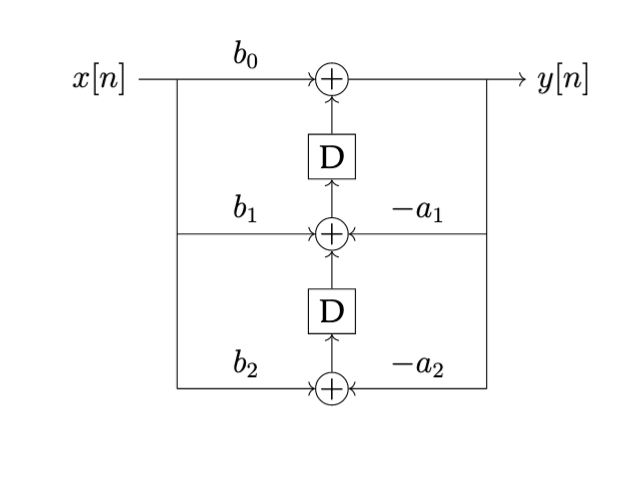
\includegraphics[scale=0.8]{diagram.png}
	\end{center}

	\begin{solution}
		I believe that the equation for this block diagram is as follows:
		\[
			y[n] + a_1y[n-1] + a_2y[n-2] = b_0x[n] + b_1x[n-1] + b_2x[n- 2]
		\] 
		this means that using the equation in the previous problem, the \( z \)-transform of this is 
		given by:
		\[
		H(z) = \frac{b_2z^{-2} + b_1z^{-1} + b_0}{a_2z^{-2} + a_1z^{-1} + 1}
		\] 
	\end{solution}
	\pagebreak
	\section*{Problem 5}
	The following pole-zero diagram belongs to a BIBO stable system \( H \) whose transfer function \( \hat{H} \)
	is rational in \( z \), and whose impulse response \( h \) satisfies:
	\[
		\sum_{n=-\infty}^{\infty} h[n] = 1
	\] 
	\begin{center}
		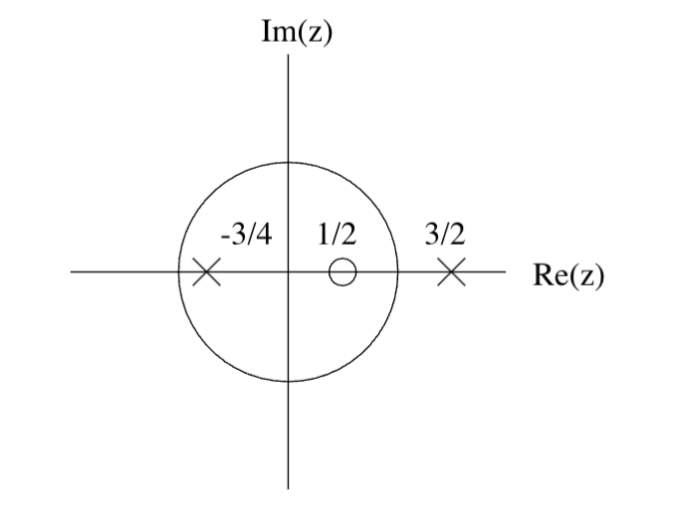
\includegraphics[scale=0.8]{diagram2.png}
	\end{center}
	\begin{enumerate}[label=\alph*)]
		\item Determine  \( h[n] \), \( \forall n \in \Z \). 

			\begin{solution}
				We know that \( H(z) \) has poles at \( z = \frac{3}{2}, z = -\frac{3}{4} \), and a zero 
				at \( z = \frac{1}{2} \). Therefore, \( H(z) \) is of the form:
				\[
				H(z) = \frac{A(1 - \frac{1}{2}z^{-1})}{(1 + \frac{3}{4}z^{-1})(1 - \frac{3}{2}z^{-1})}
				\] 
			\end{solution}
		\item Determine whether there exists a stable, causal system whose impulse response \( h_1 \) satisfies 
			\( (h * h_1)[n] = \delta[n] \). If so, specify the pole-zero diagram and the ROC for \( \hat{H}_1 \), 
			the \( z \)-transform of \( h_1 \). If not, explain briefly why no such system exists. 

			\begin{solution}
				In \( z \)-space, we know that convolution is just multiplication, so we want to find a 
				transfer function:
				\[
				H(z) H_1(z) = 1
				\] 
				Therefore:
				\[
				H_1(z) = \frac{1}{H(z)} = 
				\frac{1}{A}\frac{(1 + \frac{3}{4}z^{-1})(1 - \frac{3}{2}z^{-1})}{1 - \frac{1}{2}z^{-1}}
				\] 
				We can have this transfer function have \( |z| > \frac{1}{2} \), so all poles are within the 
				ROC, and we want the system to be causal (i.e. right sided), so therefore our system 
				could be of the form:
				\[
					h_1[n] = \frac{1}{A}\left( \frac{1}{2} \right)^{n}u[n]
				\] 
				The pole-zero plot along with the ROC for \( \hat{H_1} \) is as follows:
				\begin{center}
					\begin{tikzpicture}
						\draw[thick] (-3, 0) -- (3, 0) node[above right] {\( \Re(z) \) };
						\draw[thick] (0, -3) -- (0, 3) node[above right] {\( \Im(z) \) };
						\draw (0, 0) circle (1); 
						\filldraw[red] (1.5, 0) circle (0.05) node[above] {\small{\( z = \frac{3}{2} \) }};
						\filldraw[red] (-0.75, 0) circle (0.05) node[above] {\small{\( z = -\frac{3}{4} \) }};
						\filldraw[blue] (0.5, 0) circle (0.05) node[below] {\small{\( z = \frac{1}{2} \) }};
						\filldraw[opacity= 0.3, pattern = north west lines, even odd rule, color = orange] 
							(0,0) circle (0.5) (-3, -3) rectangle (3, 3);
					\end{tikzpicture}
				\end{center}
				the orange shaded area denotes the region of convergence, and the red and blue dots denotes 
				the poles and zeroes, respectively.
			\end{solution}
		\item Determine whether there exists a sytsem whose impulse response \( h_2 \) is left sided and 
			satisfies \( (h * h_2)[n] = \delta[n] \). If so, specify the pole-zero diagram and the ROC for 
			\( \hat{H}_2 \), the \( z \)-transform of \( h_2 \). If not, explain briefly why no such system exists. 

			\begin{solution}
				The equation is the same, so we want \( |z| < \frac{1}{2} \), and our \( h_2[n] \) is:
				\[
					h_2[n] = \frac{1}{A}\left( \frac{1}{2} \right)^{n}u[-n - 1]
				\] 
				The pole-zero diagram for \( \hat{H_2} \) is:
				\begin{center}
					\begin{tikzpicture}
						\draw[thick] (-3, 0) -- (3, 0) node[above right] {\( \Re(z) \) };
						\draw[thick] (0, -3) -- (0, 3) node[above right] {\( \Im(z) \) };
						\draw (0, 0) circle (1); 
						\filldraw[red] (1.5, 0) circle (0.05) node[above] {\small{\( z = \frac{3}{2} \) }};
						\filldraw[red] (-0.75, 0) circle (0.05) node[above] {\small{\( z = -\frac{3}{4} \) }};
						\filldraw[blue] (0.5, 0) circle (0.05) node[below] {\small{\( z = \frac{1}{2} \) }};
						\filldraw[opacity=0.3, pattern = north west lines, color=orange] (0, 0) circle (0.5);
					\end{tikzpicture}
				\end{center}
				the orange shaded area denotes the region of convergence, and the red and blue dots denotes 
				the poles and zeroes, respectively.
		\end{solution}
		\item Consider a complex DT function \( g \) related to \( h \) according to the relationship
			\[
				g[n] = z_0^{n}h[n], \ \forall n
			\] 
			where \( z_0 \) is a non-zero complex number. Hence, \( z_0 \) can be expressed in polar form 
			as \( z_0 = r_0e^{i \omega_0} \), where \( r_0 \) and \( \omega_0 \) are real, \( r_0 > 0 \) 
			and \( -\pi < \omega_0 < \pi \). If \( g \) is the impulse response of a discrete-time LTI system \( G \), 
			specify all values of \( r_0 \) and \( \omega_0 \) for which the system \( G \) would be stable. 

			\begin{solution}
				Using the \( z \)-transform properties (specifically scaling), we know that:
				\[
				G(z) = H(\frac{z}{z_0})
				\] 
				The region of convergence would scale by \( |z_0| = r_0 \). Based on the slides, we know that 
				a system is stable if and only if all the poles lie within the unit circle. What this implies, 
				effectively, is that the size of the radius of convergence must contain the unit circle. Once it leaves 
				the unit circle, it implies the existence of a pole outside the unit circle, and hence our system is 
				no longer stable. 

				The current ROC is given as \( |z| > \frac{1}{2} \), meaning that since the updated ROC is 
				\( r_0|z| > \frac{1}{2} \), then we require that \( |z| > \frac{1}{2r_0} \) and we want to 
				enforce that:
				\[
				\frac{1}{2r_0} > 1
				\] 
				This implies that all values \( r_0 < \frac{1}{2} \) are valid. 
			\end{solution}
	\end{enumerate}

	\pagebreak
	\section*{Problem 6}
	Consider a discrete-time LTI system with system function that has the following algebraic form (for all \( z \) in 
	an appropriately-defined ROC):
	\[
	\hat{H}(z) = \frac{1}{(1 - \frac{1}{2}z^{-1})(1 + \frac{1}{3}z^{-1})(1 - 2z^{-1})}
	\] 
	\begin{enumerate}[label=\alph*)]
		\item Draw the pole-zero diagram for \( \hat{H} \). 

			\begin{solution}
				There are no zeros for \( \hat{H} \), only poles, so therefore the diagram looks like:
				\begin{center}
					\begin{tikzpicture}
						\draw[thick] (-3, 0) -- (3, 0);
						\draw[thick] (0, -3) -- (0, 3) node[right] {\( \hat{H}(z) \) };
						\filldraw[red] (2, 0) circle (0.05) node[above] {\small{\( z = 2 \) }};
						\filldraw[red] (0.5, 0) circle (0.05) node[above] {\small{\( z = \frac{1}{2} \) }};
						\filldraw[red] (-0.33, 0) circle (0.05) node[above left] {\small{\( z = -\frac{1}{3} \) }};
					\end{tikzpicture}
				\end{center}
				the red dots denote the location of the poles. 
			\end{solution}
		\item Suppose we are told that the system is stable. Could it also be causal? Briefly justify your answer. 

			\begin{solution}
				We know that a causal LTI system is stable if and only if all its poles lie inside the unit circle. 
				Here, we have a pole at \( z = 2 \), which lies outside the unit circle, so even if the 
				system is stable, it cannot be causal. 
			\end{solution}
		\item Suppose instead that we are given the following candidate forms for the impulse response of the system.
			The exact values of the non-zero constants  \( A, B, \dots \) are not important for this problem, and 
			need not be determined. 

			For each candidate impulse repsonse, determine if it could or could not be the impulse response 
			of the system, and if it could, determine the ROC of \( \hat{H} \) which is consistent with that 
			particular form for the impulse response. If the candidate response could not be the 
			impulse response, briefly explain why. 
			\begin{align*}
				h_1[n] &= A\left( \frac{1}{2} \right)^{n} u[n] + b\left( \frac{1}{4} \right)^{n}u[n] + 
				C 2^{n}u[n] \\
				h_2[n] &= D\left( \frac{1}{2} \right) ^{n}u[n] + E\left( -\frac{1}{3} \right) ^{n}u[n] + F 2^{n}
				u[n]\\
				h_3[n] &= G\left( \frac{1}{2} \right)^{n}u[-n -1] + H\left( -\frac{1}{3} \right)^{n}u[n] + I 2^{n}
				u[-n - 1]\\
				h_4[n] &= J \left( \frac{1}{2} \right) ^{n}u[n] + K\left( -\frac{1}{3} \right) ^{n}u[-n - 1] + 
				L 2^{n}u[-n - 1]\\
			\end{align*}

			\begin{solution}
				I'll just go down the line: 
				\begin{itemize}
					\item \( h_1[n] \) cannot be, since the coefficients which are exponentiated
				in \( h_1[n] \) are not the poles of \( \hat{H}(z) \), hence they cannot match. 
					\item \( h_2[n] \) works for the system, and this is specifically the case where 
				we have the ROC extend towards infinity, or in other words \( h[n] \) is right-sided. The ROC in this 
				case would be \( |z| > 2 \), since \( z = 2 \) is the outermost pole. 
			\item \( h_3[n] \) has the proper roots. The step functions tell us that \( |z| < \frac{1}{2} \), 
				\( |z| > \frac{1}{3} \) and \( |z| < 2 \). The last inequality is rather useless, but the intersection 
				of all three gives us the ROC: \( \frac{1}{3} < |z| < \frac{1}{2} \)
			\item \( h_4[n] \) \textit{almost works}, except for the fact that the region of convergence for 
				this \( h[n] \) is the null set. In other words, there are no values of \( |z| \) such that 
				the \( z \)-transform converges, hence this cannot be a valid impulse response. 
				\end{itemize}			
			\end{solution}
		\item What is the constant-coefficient difference equation governing the discrete-time LTI system whose transfer
			function is characterized by \( \hat{H}(z) \)?

			\begin{solution}
				The constant-coefficient difference equation can be found by expanding the denominator. I used 
				mathematica to do the expansion becuase I got lazy, and it gives us:
				\[
				H(z) = \frac{1}{1 - \frac{1}{3}z^{-3} - \frac{1}{2}z^{-2} + \frac{11}{6}z^{-1}}
				\] 
				this implies that \( b_0 = 1 \), \( a_0 = 1, a_1 = \frac{11}{6}, a_2 = -\frac{1}{2}, 
				a_3 = -\frac{1}{3} \). Therefore, the difference equation is:
				\[
					y[n] + \frac{11}{6}y[n - 1] - \frac{1}{2}y[n - 2] - \frac{1}{3}y[n - 3] = x[n]
				\] 
			\end{solution}
	\end{enumerate}

	\pagebreak
	\section*{Problem 7 (Optional)}
	You are given the following pieces of infomration about a real, finite-valued discrete-time signal \( x[n] \) 
	 and its DTFT \( X(e^{j \omega}) \), which can be writen in teh form
	 \[
	 X(e^{j \omega}) = A(e^{j \omega}) e^{j \theta_x (e^{j \omega})}
	 \] 
	 The function \( A(e^{j \omega}) \) is periodic, real-valued \textit{amplitude} function, related to the 
	 magnitude of the DTFT \( |X(e^{j \omega})| \) by \( A(e^{j \omega}) = |X(e^{j \omega})| \). The periodic 
	 function \( \theta_x(e^{j \omega}) \) represents an angle. 
	 \begin{enumerate}[label=\alph*)]
		 \item \( x[n] \) is a finite-length signal
		 \item The \( z \)-transform \( \hat{X}(z) \) has exactly two poles, both at \( z = 0 \) (and no 
			 zeros at \( z = 0 \)). 
		 \item \( \theta_x(e^{j \omega}) = \begin{cases}
				 \omega / 2 + \pi / 2, & 0 < \omega < \pi\\
				 \omega / 2 - \pi / 2, & -\pi < \omega < 0
		 \end{cases} \)
	 \item \( X(e^{j \pi}) = 2 \) 
	 \item \( \int_{-\pi}^{\pi} \left[ \dv{X(e^{j \omega})}{\omega} \right] = 2\pi j \)
	 \item The signal \( v[n] \) whose DTFT is \( V(e^{j \omega}) = \Re \{X (e^{j \omega})\}  \) satisfies 
		 \( v[2] = 2 / 3 \).
	 \end{enumerate}
	 By interpreting the pieces of information adn putting them together, determine and sketch \( x[n] \). You may 
	 continue to use the space on the following page to show your work. 
\end{document}
